\documentclass[final,oneside,onecolumn,12pt,a4paper]{book}%
%薛丞宏加的
\usepackage{fontspec} 
\usepackage{xeCJK} 
\usepackage{ruby}
\XeTeXlinebreaklocale "zh" 
\XeTeXlinebreakskip = 0pt plus 1pt 
\renewcommand{\rubysep}{-4ex}
\pagestyle{empty}
%Select fonts
%\setmainfont[Mapping=tex-text]{Times New Roman} % rm
%\setsansfont[Mapping=tex-text]{Arial}           % sf
%\setmonofont{Courier New}                       % tt
\setCJKmainfont{DFKai-SB} %xelatex 標楷體
\setCJKmonofont{MingLiU}  %xelatex 細明體
\linespread{3}

\makeatletter
\newcommand{\rubybot}[2]{%
  \@tempdimc \f@size\p@
  \begin{tabular}[t]{@{}c@{}}
    #1\\[-3em]
    \fontsize{.8\@tempdimc}{.8\@tempdimc}\selectfont%
    \setlength{\normalbaselineskip}{0pt}#2 
  \end{tabular}%
}
\makeatother
\usepackage[toc,page]{appendix}
\usepackage{makecell}
%薛丞宏加的

\usepackage{amsmath}
\usepackage{amsfonts}
\usepackage{amssymb}
\usepackage{url}
\usepackage{hyperref}
\usepackage{algorithm}
\usepackage{algorithmic}
\usepackage{graphicx}%
\setcounter{MaxMatrixCols}{30}
\usepackage[left=3cm, right=2cm, top=2.5cm, bottom=2.5cm]{geometry}
%TCIDATA{OutputFilter=latex2.dll}
%TCIDATA{Version=5.50.0.2953}
%TCIDATA{Created=Monday, May 12, 2003 22:46:51}
%TCIDATA{LastRevised=Friday, August 30, 2013 14:39:59}
%TCIDATA{<META NAME="GraphicsSave" CONTENT="32">}
%TCIDATA{<META NAME="SaveForMode" CONTENT="1">}
%TCIDATA{BibliographyScheme=BibTeX}
%TCIDATA{<META NAME="DocumentShell" CONTENT="Standard LaTeX\Blank - Standard LaTeX Article">}
%TCIDATA{Language=American English}
%TCIDATA{PageSetup=72,72,72,72,0}
%TCIDATA{Counters=arabic,1}
%TCIDATA{AllPages=
%H=36
%F=36
%}
%BeginMSIPreambleData
\providecommand{\U}[1]{\protect\rule{.1in}{.1in}}
%EndMSIPreambleData
\oddsidemargin 0.0in
\textheight=8.5in
\textwidth=6.5in
\headheight=0.0in
\topmargin=0.0in
\newtheorem{theorem}{Theorem}
\newtheorem{abstract}{abstract}
\newtheorem{acknowledgement}[theorem]{Acknowledgement}
\newtheorem{axiom}[theorem]{Axiom}
\newtheorem{case}[theorem]{Case}
\newtheorem{claim}[theorem]{Claim}
\newtheorem{conclusion}[theorem]{Conclusion}
\newtheorem{condition}[theorem]{Condition}
\newtheorem{conjecture}[theorem]{Conjecture}
\newtheorem{corollary}[theorem]{Corollary}
\newtheorem{criterion}[theorem]{Criterion}
\newtheorem{definition}[theorem]{Definition}
\newtheorem{example}[theorem]{Example}
\newtheorem{exercise}[theorem]{Exercise}
\newtheorem{lemma}[theorem]{Lemma}
\newtheorem{notation}[theorem]{Notation}
\newtheorem{problem}[theorem]{Problem}
\newtheorem{proposition}[theorem]{Proposition}
\newtheorem{remark}[theorem]{Remark}
\newtheorem{solution}[theorem]{Solution}
\newtheorem{summary}[theorem]{Summary}
\interdisplaylinepenalty=2500
\sloppy
\pagenumbering{arabic}
\pagestyle{plain}
\renewcommand{\baselinestretch}{2}
\begin{document}

\frontmatter
\chapter{踏頭話}
勞力~~
\newpage

\chapter{摘要}
謝謝

\newpage

\chapter{Abstract}

Thank you

\newpage

\tableofcontents
\listoffigures
\listoftables



\mainmatter


\chapter{研究背景}
\label{章:研究背景}

\rubybot{臺 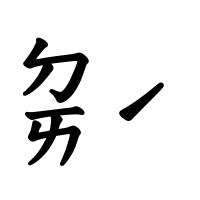
\includegraphics[height=1em]{圖/⿳⿳ㄉㄞˊ}}{tai5}
\rubybot{語 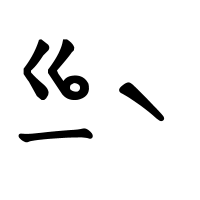
\includegraphics[height=1em]{圖/⿳⿳ㆣㄧˋ}}{gi2}
媠\footnote{\rubybot{臺 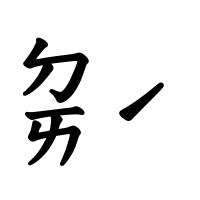
\includegraphics[height=1em]{圖/⿳⿳ㄉㄞˊ}}{tai5}}

為著格式一致,全部轉臺羅,人名、文章名、冊名保持原樣

\section{臺語介紹}
\label{章:臺語介紹}

\section{語料狀況}
\label{節:語料狀況}

The rest of this paper is organized as follows. Chapter
\ref{章:相關研究} covers some preliminaries.
The three versions of the PTI discovery problem are formulated in Chapter
\ref{章:臺語介紹}. Chapter \ref{章:翻譯語料} presents our
solutions based on the shockwave approach. Our field trial and simulation
results are provided in Chapter \ref{章:摻猶未整理語料} and
\ref{章:網路語料庫}. Conclusions and future works are drawn in Chapter
\ref{章:結論佮未來發展}.

\chapter{相關研究}
\label{章:相關研究}


\chapter{翻譯語料}
\label{章:翻譯語料}

頂一章有講

\section{新聞語料庫}
\label{節:新聞語料庫}
華語臺語雙語語料庫\footnote{\url{http://icorpus.iis.sinica.edu.tw/}}(後壁用「新聞語料庫」稱呼)是何澤政\footnote{一九七零年代出世,臺中烏日人}對民國九十七年十一月初六開始,逐工揣兩篇國語新聞,先斷句,後尾翻譯做臺語教會全羅。親像原本的新聞「這幾天寒流再度發威」,翻譯做「tsit4-kui2-kang han5-liu5 koh-tsai3 tian2-ui」(這幾工寒流閣再展威)\footnote{原文是教會羅馬字,為著文章一致,以教育部的臺羅書寫}。
新聞語料庫的翻譯罕得改變用詞的先後,親像面頂的「這幾天寒流再度發威」,較袂翻做「寒流這幾工閣再展威」,除非照國語用詞先後翻譯的結果無順,才會調整。

澤政佇語料內底用
「挕捒 hinn3-sak4」\footnote{挕捒意思共物件擲掉、放捒,嘛就是華話的「丟棄」,例句甲(家己做的):這支筆好好,為啥物愛共伊挕捒。例句乙(Tek-hôa,Nah ē teh批判民進黨?,\url{http://taioan-chouhap.myweb.hinet.net/089.htm}):民進黨接續李登輝的路線, 繼續加強黨國時代權力者, 倚附者佮既得利益者的優勢,毋是共刜挕捒。}
、
「作孽」\footnote{
青-少-年|tshing1-siau3-lian5 作-孽|tsok4-giat8 跤-踏-車|kha1-tah8-tshia1 擲|tan3 落|loh8 河-中|ho5-tiong1。

愛耍手賤,華語的「惡作劇」。例句甲:叫你莫摸你閣摸,誠實手賤愛作孽!(家己做的)例句乙:你這个作孽囡仔,你是按怎沐甲一身軀烏趖趖?(惠光,天真瀾漫,\url{http://ip194097.ntcu.edu.tw/nmtl/DADWT/thak.asp?id=992})}
本土的詞以外,伊嘛會配合這馬發生的代誌,用較時行的臺語,親像
「喙罨」\footnote{華語的「口罩」}、
「心肌梗窒」\footnote{心|sim1 肌|ki1 梗|king2 窒|that4,華語的「心肌梗塞」}、
「自來水」\footnote{臺語較古典的用法,會號做「水道水」}、…。
而且除了現代臺語,澤政伊閣會去查台華線頂辭典\footnote{\url{http://ip194097.ntcu.edu.tw/iug/Ungian/SoannTeng/chil/Taihoa.asp}}
選擇較古典的用詞\footnote{台華線頂辭典是古早語料,一个詞若台華線頂辭典查有,教育部辭典查無,就當做伊是較古典的詞},親像
「𤺪|sian7 篤-篤|tauh4-tauh4」\footnote{熱-天|juah8-thinn1 高-溫|ko1-un1 炎-熱|iam7-juah8 規-工|kui1-kang1 𤺪|sian7 篤-篤|tauh4-tauh4 。|。}、「鬥-贊-手|tau3-tsan3-tshiu2」\footnote{佇|ti7 三|sam1 一-一|it4-it4 大-地-動|tua7-te7-tang7 慷-慨|khong2-khai3 鬥-贊-手|tau3-tsan3-tshiu2 ,|,}。

拄著外來詞,澤政嘛會選擇保留原文,拄著國語的「歐巴馬」佮「西藏」,會翻轉去英文「Obama」、「Tibet」。

斷詞組

加漢字,

若源頭是日本話外來詞,就會直接用教羅寫出來,請看

\section{翻譯架構}
\label{節:翻譯架構}
國語翻譯到臺語需要兩項物件,一項是國語翻譯到臺語的語詞對照表,另外一項是知影臺語逐句好歹的語言模型。這馬時行的翻譯系統是統計翻譯(statistical machine translation),會當分做三个部份:

第一个是對齊模型(alignment model),負責產生語詞對照表,逐擺提一組國語佮臺語的平行語料出來,親像「我 要 吃飯」和「我 欲 食 飯」,國語詞的「要」,會對應到「我」、「欲」、「食」、「飯」臺語詞,經過大量的平行語料,上尾知影國語的「要」定定對應著臺語的「欲」,也就是共對應頻率懸的組合留落來。

第二部份是語言模型(language model),伊去記錄逐个詞後壁定定會接啥物詞,若有一句話是「…欲 食…」,有「欲」佮「食」兩个詞,咱知影「…欲 食」的後壁接「飯」比「…欲 食」的後壁接「湯」的機率較大,也就是講「欲 食 飯」連紲詞比「欲 食 湯」連紲詞機率大,若語言模型一擺看「欲 食 飯」三个詞,就是三連紲詞模型(3-grams model)。語言模型判斷一句話,伊出現的機率有偌大,就是看這句話伊內底連紲詞的機率是偌大。

上尾一部份是解碼器(decoder),提面頂講的對齊模型、語言模型,來翻譯國語到臺語。因為翻譯的問題毋是多項式時間(NP problem)會當解出來的,所以解碼器袂使硬算全部的可能,必須用有效率的演算法來翻譯。

\section{評分方式}
\label{節:評分方式}

翻譯大部份攏用BLEU(Bilingual Evaluation Understudy)來評分\footnote{\url{https://github.com/moses-smt/mosesdecoder/blob/master/scripts/generic/multi-bleu.perl}},伊用連紲詞的概念來評分,$BLEU=100\times{e^{\max{0,\frac{\textit{結果-答案長度}}{\textit{結果長度}}}}}\times{\sum_{n=1}^{4}(\textrm{n連紲詞})^{\frac{1}{4}}}$。

準若翻譯的答案是「這 幾 工 寒流 閣再 展威」,咱有兩个翻譯的結果,翻譯結果一「這 幾 工 寒流 有 展威」佮結果二「寒流 這 幾 工 閣再 展威」,請看表\ref{表:範例BLEU分數},答案有「這 幾 工」、「幾 工 寒流」、「工 寒流 閣再」佮「寒流 閣再 展威」4个三連紲詞,結果一有出現2个,所以結果一的三連紲詞分數是2/4,結果二有出現1个,分數是1/4。因為結果二無對應的四連紲詞,伊的分數都比結果一低。

\begin{table}
\caption{翻譯結果一「這 幾 工 寒流 有 展威」佮翻譯結果二「寒流 這 幾 工 閣再 展威」對答案「這 幾 工 寒流 閣再 展威」的分數}%
\label{表:範例BLEU分數}
\centering
\begin{tabular}{|c|cccc|c|}
\hline
翻著的數量 & 一連紲詞 & 兩連紲詞 & 三連紲詞 & 四連紲詞 & BLEU分數\\
\hline
結果一 & 5/6 & 3/5 & 2/4 & 1/3 & 53.73\\
\hline
結果二 & 6/6 & 3/5 & 1/4 & 0/4 & 0.00\\
\hline
\end{tabular}
\end{table}


\section{未知詞問題}
\label{節:未知詞問題}
系統結構會當看圖,語言模型用Witten-Bell加discounting的算法,翻譯模型用預設的參數。

訓練語料用新聞語料庫頭前2300篇新聞,攏總57167句,試驗語料用上尾267篇新聞,攏總6954句。按呢無調整語料,直接照伊的斷詞組落去訓練,共結果佮答案一句內底拆做一字一字,用\ref{節:評分方式}的BLEU去算分數,得著70.67分。

詳細看分數歹的原因,是因為傷濟詞組佇訓練語料無出現過,親像提原本試驗語料的華語句「陸續 開放 一百五十項 的 規費」去翻譯,得著「liok8-siok8 khai1-hong3 一百五十項 e5 規費」 ,「一百五十項」無翻譯出來,是因為訓練語料內底無出現過這个詞組,對訓練語料來講,「一百五十項」就是一个未知詞組。但是訓練語料內底有「兩項」佮「一百五十位」的華語詞組,煞無法度提來用。

為著予翻譯的結果閣較好,按算用兩種方式來加強未知詞的處理,頭一个是改變翻譯的單位,共原本斷詞組的語料改做斷詞抑是斷字,寫佇\ref{節:改變語料格式}節。第二个方法仝款照斷詞組翻譯,若拄著未知詞,針對未知詞專工處理,會當看\ref{節:未知詞另外翻譯}節。



\section{改變語料格式}
\label{節:改變語料格式}

頂一節發覺若用詞組當做翻譯的單位,會因為詞組單位傷大,變做真濟詞組無看過。所以咱都共華語佮臺語攏用一字一字做翻譯的單位,共原本的「陸續 開放 一百五十項 的 規費」,變做「陸 續 開 放 一 百 五 十 項 的 規 費」。照按呢共訓練語料變做一字一字,共這句翻譯會當得著「陸|liok8 續|siok8 開|khai1 放|hong3 一|tsit8 百|pah4 五|goo7 十|tsap8 項|hang7 的|e5 規|kui1 費|hui3 ,|,」,效果比原本斷詞組的閣較好,得著82.94分。

語料格式的影響著翻譯的效果,除了斷字,翻譯嘛會使用斷詞做單位,華語用中研院中文斷詞系統(CKIP)\footnote{\url{http://ckipsvr.iis.sinica.edu.tw/}}斷詞,臺語用辭典斷詞\footnote{實際按怎做請看\ref{節:斷詞方法}}。「」提去翻譯會得著「」。斷詞的分數是76.88分,比斷詞組閣較好一寡,毋過小較輸斷字。三个分數整理佇表\ref{表:斷詞組、斷詞、斷字做單位的翻譯分數}。

\begin{table}
\caption{斷字、斷詞佮斷詞組做單位的分數}%
\label{表:斷詞組、斷詞、斷字做單位的翻譯分數}
\centering
\begin{tabular}{c|ccc}
翻譯單位 & 斷字 & 斷詞 & 斷詞組\\
\hline
分數 & 82.94 & 76.88 & 70.67\\
\end{tabular}
\end{table}

\section{未知詞另外翻譯}
\label{節:未知詞另外翻譯}

對頂頭的結果來看,用斷字來做翻譯較袂拄著未知詞的問題。換別的角度來看,準若咱用斷詞組的翻譯模型,拄著未知詞的時陣,這个未知詞會使提予斷字翻譯模型去翻譯,就是講「陸續 開放 一百五十項 的 規費」提予斷詞組模型翻譯,得著「liok8-siok8 khai1-hong3 一百五十項 e5 規費」,閣來共「一百五十項」佮「規費」這兩个詞組切做斷字「一 百 五 十 項」佮「規 費」,閣擲去斷字模型翻譯,流程會當看圖XX,按呢得著84.85分。

毋過按呢閣無夠,\ref{節:改變語料格式}節的結果證明仝一份語料無仝形式會有無仝的結果,所以閣愛看覓佇斷詞、斷字的情形之下,翻譯效果是按怎變化的。

咱做的是華語翻譯到臺語,攏總兩个語言,逐个語言有斷詞組、斷詞佮斷字三種方法,實驗都有$3^{2}=9$組合,分數請看表\ref{表:華語臺語逐種形式,而且未知詞提予斷字模型翻譯的結果}。
全部分數上懸的是華語斷詞組對臺語斷詞組,原因是伊斷的詞組,對訓練翻譯模型需要對齊模型的語詞對照表\footnote{若袂記得,請看\ref{節:翻譯架構}節的說明}有幫助。
而且毋管臺語的狀態,華語斷詞攏比華語斷字閣較好,因為中研院中文斷詞系統會共定定用的詞組當作詞,親像「看 書」因為是定用詞組,會合做伙做「看書」,看無遐爾用著的「看 電視」猶原是「看 電視」。

毋過臺語斷字變斷詞了後,效果煞較禾黑,是因為臺語斷詞干焦用辭典\footnote{實際按怎做請看\ref{節:斷詞方法}}爾爾,而且詳細去比較「華語斷詞-臺語斷字」佮「華語斷詞-臺語斷詞」的結果,6954句內底有1367句無仝,用人工看頭前151組無仝的結果,逐組揀1个較好的。有71組是斷字的結果較好,有56組是斷詞模型較好,賰的24組是口腔無仝,當做是平平仔好。
閣去查斷詞為啥物翻譯較禾黑,詳細看原本斷詞的內容,「遊|iu5 客-人|kheh4-lang5 數|soo3」斷做「遊|iu5 客-人|kheh4-lang5 數|soo3」,都有淡薄仔問題矣,才會拖著翻譯效果。
%會使講準做「華語斷詞-臺語斷字」的分數比「華語斷詞-臺語斷詞」較懸,毋過人來看,煞無一定是按呢。


\begin{table}
\caption{華語臺語逐種形式,而且未知詞提予斷字模型翻譯的結果}%
\label{表:華語臺語逐種形式,而且未知詞提予斷字模型翻譯的結果}
\centering
\begin{tabular}{c|ccc}
\diaghead{\theadfont Diag ColumnmnHead II}%
{華語形式}{臺語形式} & 斷字 & 斷詞 & 斷詞組\\
\hline
斷字 & 82.94 & 82.75 & 80.61\\
斷詞 & 84.27 & 84.05 & 82.89\\
斷詞組 & 84.05 & 83.90 & 84.85\\
\end{tabular}
\end{table}

\section{語料形式選擇}
\label{節:語料形式選擇}
咱若共\ref{節:改變語料格式}節佮\ref{節:未知詞另外翻譯}節的方法合做伙,效果上好的是斷詞組對斷詞組,毋過斷詞組需要用剖析器去揣結構樹,閣來定規則決定詞佮詞啥物時陣愛敆做伙變詞組,這就是另外一門學問矣。目前臺語閣無這資源,自然賰「華語斷詞-臺語斷字」佮「華語斷詞-臺語斷詞」上好,準若有好的斷詞工具,臺語斷詞模型應該愛比臺語斷字模型閣較好,雖然佇這擺實驗斷詞模型顛倒較禾黑,毋過為著未來臺語的斷詞研究方便比較,後壁的實驗模型攏是用「華語斷詞-臺語斷詞」。

\chapter{摻猶未整理語料}
\label{章:摻猶未整理語料}
對於定定百萬句的翻譯來講傷少
加入其他的語料
教育部語料
數位典藏
 語料之間的問題
用字無一致
毋是一對一
斷詞方法無一致

\section{教育部語料佮數位典藏}
\label{節:教育部語料佮數位典藏}

\section{漢羅全羅對齊}
\label{節:漢羅全羅對齊}

\section{斷詞方法}
\label{節:斷詞方法}

\section{實驗流程佮結果}
\label{節:實驗流程佮結果}


\chapter{網路語料庫}
\label{章:網路語料庫}
現況
\section{TGB通訊-臺灣組合}
\label{節:TGB通訊-臺灣組合}

\section{語言判斷}
\label{節:語言判斷}

\section{實驗結果}
\label{節:實驗結果}


\chapter{結論佮未來發展}
\label{章:結論佮未來發展}

\chapter{--其他--}
To find $T$, we try to approximate a (real-value) GCD of $D=\left\{
T_{1},T_{2},...,T_{n-1}\right\}  $. This is done by running the DBSCAN
(Density Based Spatial Clustering of Applications with Noise) clustering
algorithm \cite{Ester1996DBSCAN} to group data items and filter out noise,
followed by a testing process to find $T$. There are several parameters used
in this approach:

In the simulations, VISSIM \cite{Mosseri2004VISSIM} was used to simulate
vehicle traffic. The Poisson arrival model with rates 18/20/24 vehicles per
minute was used to generate traffic flows into a signalized road section of
$650$ m from A to B as illustrated in Fig. \ref{fig:f_map} for $40$ minutes,
and the Wiedemann 99 car following model \cite{Mosseri2004VISSIM} was used to
depict the trajectories of vehicles. In the free flow state, vehicles move in
a range of speed between $48$ km/h and $58$ km/h. When encountering a red
signal, vehicles slow down and eventually stop. After the signal turned to
green, vehicles accelerate and then enter the free flow state.
\begin{figure}[pth]
\centerline{\includegraphics[angle=0, width=3.5in,keepaspectratio,clip]
{figures/f_map.eps}} \hfill\caption{The road segment in simulation and field
trial experiments. B is the location of the traffic light.}%
\label{fig:f_map}%
\end{figure}

\bibliographystyle{IEEEtran}
\bibliography{翻譯論文}

\begin{appendices}
\chapter{Some Appendix}
\chapter{Some Appendix}
The contents...
\end{appendices}

\end{document}